\section{Introduction}
\label{sec:intro}

%\KZ{Add citations wherever possible, e.g., when you talk about coming
%relatedness on taxonomy or co-occurrence.}
Computing semantic relatedness between two terms or concepts has been
an essential problem in data mining and natural language processing (NLP),
because relatedness is frequently used in many applications
such as information retrieval, recommendation systems, question answering
and human computer interaction.
%\KZ{cite the applications here as well.}
Traditionally, relatedness has been explored in the context of
semantic {\em similarity}. Strictly speaking, there are two types
of similarity. One measures the degree of {\em commonality}
between two objects, e.g., football and soccer;
the other estimate the degree of {\em association}
between two objects, e.g., soccer and World Cup. The first type of similarity
is usually computed with the help of a taxonomy system such as WordNet
\cite{Resnik:1995,Jiang:1997,Lin:1998} or Probase \cite{LiWZWW13}.
The second type is commonly referred to as relatedness or,
loosely speaking, association. Relatedness, on the other hand, has been
computed from distributional properties from large text corpora
\cite{StrubeP06,ChenLW06,GabrilovichM07,BollegalaMI11a}.
Some of the corpora used include web text \cite{LiPeipei:2013}, search engine snippets
\cite{Sahami:2006} and Wikipedia articles \cite{Gabrilovich:2007}.
The primary feature used in all these systems is
{\em term-term co-occurrence} information. That is, two terms
are considered related, {\em if and only if} they co-occur frequently
within a window in a document. Such window can be a sentence, a paragraph,
or a document.
Because the above definition of relatedness rely heavily on
the number of co-occurrences, it does not work very well when the
corpus is not large enough and thus the sample of co-occurrences
doesn't correspond to the real distribution.
In other words, previous work merely attempts to derive
the strength of direct connection between two concepts, ignoring the fact
that two concepts might be connected not through direct co-occurrence, but
only through a number of other {\em latent} concepts,
a process we call {\em mind drifting}, which will the focus of
discussion in this paper.

%Another one\cite{} uses documents or snippets returned by search engine
%as the corpus,
%and calculate term relatedness from the co-occurrence information.
%Also, there are methods use Wikipedia pages\cite{} as data source,
%and get relatedness information from the overlap of those pages.
%
%large corpus \cite{StrubeP06,ChenLW06}, no matter how weak the relatedness is.
%There are several typical types of traditional methods to compute word relatedness or similarity,
%one relies on taxonomy system like WordNet,
%and use the location of the two words in the system to compute their similarity.
%
%\KZ{We should talk a bit more about existing approaches before diving into
%our own. Show a graph or some pics here to attract attention.}
\begin{figure}[th]
\centering
\epsfig{file=network.eps,width=\columnwidth}
\caption{A Fragment of the Concept Association Network}
\label{fig:can}
\shrink
\end{figure}

Our inspiration comes from the association activity in real human brain.
In human mind, the direct association from one concept to another is
limited to relatively strong connections,
while for relatively weak connections, human would probably complete
the association by ``drifting'' through other bridging concepts, where each
such bridge is a strong enough connection.
%\KZ{We need a {\bf driving example} in which you show the
%relatedness with common
%approaches and then show the latent path that we compute using our approach.
%We could use the Beckham and Spice girls example but this example must carry
%us thru the whole paper, including our discussion on the HMM, etc.}
For example, when we mention the concept ``football'',
one probably has little chance of being reminded of the pop group
``Spice Girls'', for they don't have much
in common, nor do they appear together frequently in any context.
However, it is very likely and quite natural for people to drift their mind
from ``football'' to ``David Beckham'', the world-renown British footballer,
then from ``David Beckham'' to his wife
``Victoria Beckham", and finally from ``Victoria Beckham''
to her former pop group ``Spice Girls''. This path of connection allows us
to associate seemingly remote concepts together in a concept association
network, which we call {\em MindDrifter} in this paper.
\figref{fig:can} shows a fragment of the network, where
the arrows indicate the one-way association.

%\KZ{The following para is too long.}
Looking into the mind drifting process,
we discover two important characteristics:
First, each step of the association is only affected by
the previous step, that is, the associate process is typically
a one-way chain. Second, each step of association happens under
certain context.
For example, at the mention of ``David Beckham'', Spanish sports fans
may first think of ``Real Madrid'' and the days David spent there;
while fashion and music lovers may first think of ``Victoria Beckham''
and latest news about the couple. With these two typical features,
one natural solution to model the mind drifting process is Hidden
Markov Model (HMM). That is, each state in the HMM model is the
probability distribution of every possible contexts.
And under each certain state, the observable result will be the probability of thinking of concept B at the mention of concept A under this state.
Then we can model the mind drifting process and use it to calculate the relatedness between concepts in human mind.

In order to build this concept association network under the HMM model,
we need to obtain the necessary parameters and scores from sample data,
and online encyclopedias are a good data source for information extraction
and knowledge construction. In this paper, we focus on building such an
association network for Chinese terms, and therefore, we turned our attention
to Chinese Wikipedia\cite{wikipedia}, Baidu Encyclopedia \cite{baidu-baike},
and Hudong Encyclopedia\cite{hudong-baike}, three largest online knowledge
sources in the Chinese language.
%\KZ{Show example snapshots of these encyclopedias}
Currently, these three data sources contain millions of pages.
Each page has a title, which is a word or phrase in Chinese,
representing one or more Chinese concept under the same name,
and an article with links which defines or describes the title.
While Wikipedia is familiar to most readers,
Baidu and Hudong are a little different in that they don't
have disambiguation pages, thus descriptions for each sense of the word
are all in the same page. \secref{sec:data} will explain in more
detail the characteristics of these three data sources and how we
merge them and extract the needed information to
construct the HMM model and Chinese concept association network.

%\KZ{Most audiences know
%wikipedia, so just highlight the difference between wiki and the two other
%resources briefly. We will have a separate section on these data source in
%the main part of the paper. The discussion below is a bit too detail. Leave
%it to its own section later.}

%And we can get three types of information
%from a page: the first one is the link structure, usually there are
%some words added hyperlinks to other concepts' pages in a page.
%The second one we call it "title-body co-occurrence",
%which means the co-occurrence of a title and another word
%appearing in its page. The third one is "sentence-level co-occurrence",
%representing the co-occurrence of two words in one sentence in any page.
%We see the three types of information in different way:
%the link structure means the relations of contexts drifting,
%when we click the hyperlink and enter another page from the current page,
%it can be seen as we get into another context from the previous context,
%so we use this information to get our concepts' transition matrix.
%As for the "title-body co-occurrence" and "sentence-level co-occurrence",
%we regard them respectively represents relatedness in two
%perpendicular directions. The "sentence-level co-occurrence" more
%represents relatedness in the vertical direction, that one concept
%is part or a feature of the other concept, or one concept is a generalization
%of the other concept. The association from "football" to
%"David Beckham" and that from "Victoria Beckham" to "Spice Girls"
%are more in this type of relatedness. And "sentence-level co-occurrence"
%is the relatedness in horizontal direction, that two concepts may share
%much in common, be in the same group or have close relationships,
%the association from "David Beckham" to "Victoria Beckham" are more
%in this case. And we think that when people associate from one concept
%to another, they might think vertically or horizontally, each direction
%has a probability and the ratio differs under different contexts.

%\KZ{Use one para to say what are the key technical challenges in our work.
%And then use one para to say what are our main contributions. Name 3-4
%contributions will suffice. But must distill these contributions so that they
%are sharp and to the point!}

The construction of the association network poses two
major technical challenges.
First, because of the structural differences between the three input
data sources, it is non-trivial to merge the three together to form
a unified corpus. We propose a clustering algorithm to merge articles about
identical or synonymous terms.
Second, there are two kinds of co-occurrences in the input data,
namely ``title-body'' co-occurrence and ``sentence-level'' co-occurrence which
give rise to vertical and horizontal connections, respectively,
in the association network (see \figref{fig:can}).
What is the relation between the two types of connections and
when to taken horizontal vs. vertical during relatedness computation
is a significant issue. We decided that the association process
makes a dynamic decision to drift vertically or horizontally,
each with a prior probability. We propose to learn a parameter
$\alpha$ to combine them together in a probabilistic process.
%And finally we design a way to get the parameter $\alpha$ for each context.

%table
\begin{table}[th]
\centering
\caption{Most Related Terms to ``Tiger'' and ``Planet''
under Three Relatedness Calculations}
\label{tab:comparison}
\small
\begin{tabular}{|r|r|r|}
\hline
{\bf MindDrifter} & Google & CIKM'13\\
\hline
\multicolumn{3}{|c|}{Tiger}\\
\hline
Feline & Animal & Jaguar\\
Carnivore & Fauna & Animal\\
Jaguar & Organism & Carnivore\\
Animal & Cat & Cat\\
Mammal & Feline & Mammal\\
Cat & Jaguar & Feline\\
Organism & Mammal & Organism\\
Fauna & Carnivore & Fauna\\
\hline
\multicolumn{3}{|c|}{Planet}\\
\hline
Star & Moon & Moon\\
Astronomer & Astronomer & Sun\\
Sun & Gaxaly & Star\\
Gaxaly & Star & \\
Moon & People & \\
Constellation & Sun & \\
People & Constellation & \\
Space & Space & \\
\hline
\end{tabular}
\end{table}

This paper makes three main contributions.
\begin{enumerate}
\item With relatively small but semi-structured and condensed data sources,
we have constructed a concept association network that allows us to
compute traditional similarity between terms more accurately than if
much large corpus was used.
\tabref{tab:comparison} compares MindDrifter with normalized
Google distance and a recent similarity measure called CIKM'13 \cite{LiWZWW13}
when computing the most related concepts from ``tiger'' and ``planet''.
\item Thanks to the concept association network
and HMM model, our algorithm effectively computes the best path between
two terms in the network, which may contain other terms as latent
bridge nodes. These latent nodes reveal how the two input terms
are possibly associated.
\item By using the chain of mind drifting association,
we can detect latent connection between two concepts,
and then calculate their relatedness score more precisely,
especially for weakly associated terms. Our proposed associate model
significant improve the performance of recommendation system
under the ``cold start'' situation.
\end{enumerate}

%\KZ{this para should give follow refences to the rest of the sections.}
The rest of the paper is organized as follows.
\secref{sec:data} will describe the three data sources and how we merge
them to create one unified data source. \secref{sec:approach} will
present a basic algorithm and an advanced algorithm to construct
the association network, and how to calculate relatedness using this network.
\secref{sec:eval} shows how this technology is useful in similarity
computation and recommendation systems. Finally we compare our work with
a large body of related work in \secref{sec:related} and conclude the paper
in \secref{sec:conclude}.

